\documentclass{article}
\usepackage[utf8]{inputenc}
\setlength{\parindent}{0em}
\setlength{\parskip}{1.4ex}
\usepackage[danish]{babel}
\usepackage[utf8]{inputenc}
\usepackage{graphicx}
\graphicspath{{pictures/}}
\usepackage{mathtools}
\usepackage{amsfonts,amsmath,amssymb,amsthm} 
\newtheorem{theorem}{Sætning}

\title{DM500 Eksamensopgave}

\author{
	Thomas Urup Schjerlund\\
	\texttt{thsch20@student.sdu.dk}
	\and
	Tobias Klink Lehn\\
	\texttt{toleh20@student.sdu.dk}
	\and
	Philip Hayberg Thomsen\\
	\texttt{phtho20@student.sdu.dk}
	\and
	Sean Chrone Græns\\
	\texttt{segra20@student.sdu.dk}
}
\date{15. November 2020}

\begin{document}

\begin{titlepage}
\maketitle
\end{titlepage}

\section{Reeksamen DM527 Opg 1 - Tobias}
\begin{figure}[h]
\includegraphics[scale=1]{Opgave1Formulering}
\end{figure}

\begin{figure}[h]
\includegraphics[scale=1]{opga}
\end{figure}
\textbf{Svar:}
En afbildning, $\phi: A \rightarrow B$ er bijektiv, hvis og kun hvis funktionen både er \emph{injektiv} (one-to-one) og \emph{surjektiv} (onto).

\begin{theorem}
$f$ er injektiv, hvis $\forall x_1, x_2 \in Dm(f): x_1 \neq x_2 \rightarrow f(x_1) \neq f(x_2)$
\end{theorem}

Sagt på en anden måde, så skal det for alle værdier af x i definitionsmængden gælde, at x hvis to x-værdier er forskellige fra hinanden, så er deres funktionsværdier det også. Helt basalt vil det sige, at to x-værdier ikke kan dele en y-værdi.

Ved at indsætte $x_1$ og $x_2$ og sætte deres funktionsværdi lig hinanden, kan det afgøres hvorvidt det også betyder, at x-værdierne var ens til at starte med - det skal de være, hvis funktionen skal være injektiv:
\begin{center}
\[f(x_1) = x_1^2 + x_1 + 1 \] 
\[ f(x_2)=x_2^2 + x_2 + 1 \] 
\begin{align*}
f(x_1) = f(x_2) \\
\Rightarrow x^2_1 + x_1 + 1 = x^2_2 + x_2 + 1 && \text{Funktionsværdien indsættes} \\
\Leftrightarrow x^2_1 + x_1 = x^2_2 + x_2 && \text{1 går ud på begge sider} \\
\Leftrightarrow x_1^2 = x_2^2 + x_2 - x_1 && \text{$x_1$ trækkes fra på begge sider}\\
\Rightarrow x_1 = \pm\sqrt{x_2^2 + x_2 - x_1} \\
\Rightarrow x_1 = \pm\sqrt{k}  && \text{, $k \in \mathbb{R}$}
\end{align*}
\end{center}

Da det hurtigt viser sig at $x_1 \neq k \Rightarrow f(x_1) = f(k)$, må det betyde, at $x_1$ kan have samme funktionsværdi som et andet tal (forskelligt fra $x_1$) i definitonsmængden ($Dm(f) = \mathbb{R}$), og derfor er \emph{f} ikke injektiv, og derfor automatisk heller ikke bijektiv. For at understrege pointen kan man forsøge sig med $x_1 = 4.91$ og $x_2 = -5.91$ og derfor få:

\begin{align*}
\begin{split}
f(4) = 4.91^2 + 4.91 + 1 \approx 30.02  \\
f(-5.91) = (-5.91)^2 + 5.91 + 1 \approx 30.02
\end{split}
\end{align*}
Af den grund behøver vi ikke kontrollere, om \emph{f} er surjektiv.


\begin{figure}[h]
\includegraphics[scale=1]{opgb}
\end{figure}

\textbf{Svar:} En funktion \emph{f} har en invers, hvis og kun hvis f er bijektiv. Da vi tidligere har konkluderet at \emph{f} ikke er bijektiv, må det også være tilfældet, at \emph{f} ikke er invertibel og derfor ikke har nogen invers.

\begin{figure}[h]
\includegraphics[scale=1]{opgc}
\end{figure}
\textbf{Svar:} To funktioner kan adderes ved at addere deres funktionsforskrifter ved brug af standard algebraiske regler
\begin{align*}
(f+g)(x) = f(x) + g(x) \\
\Rightarrow (f+g)(x) = (x^2 + x + 1) + (2x - 2) && \text{f og g indsættes på deres pladser} \\
= x^2 + x + 1 + 2x - 2 && \text{Parentser fjernes, da der kun indgår + mellem dem} \\
= x^2 + 3x - 1 \\
\end{align*}

\begin{figure}[h]
\includegraphics[scale=1]{opgd}
\end{figure}
\textbf{Svar:} Den sammensatte funktion $f \circ g$ beregnes på følgende vis:
\par
\begin{center}
\begin{math}
f \circ g = f(g(x))
\end{math}
\end{center}

Indsætter man $f$ i $g$ fås:
\begin{center}
\begin{align*}
g(f(x)) = g(x^2 + x + 1) \\
= 2 \cdot (x^2 + x + 1) - 2 && \text{udtrykket indsættes i g} \\
= 2x^2 + 2x + 2 - 2 && \text{Parentesen udregnes} \\
= 2x^2 + 2x
\end{align*}
\end{center}

Dette var løsningen til Opgave 1 i DM527 Reeksamen, Januar 2012.

\section{Reeksamen Februar 2015 Opg. 1 - Thomas}
\begin{figure}[h]
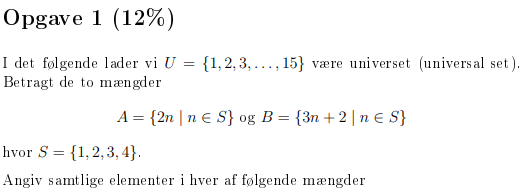
\includegraphics{2015Opgave1Formulering}
\end{figure}

\subsection*{Opgave a og b}
Vi starter med at betragte de 2 mængder \emph{A} og \emph{B}.

\begin{center}

$A = \{ 2n | n \in S \}$ \qquad $B = \{ 3n +2 | n \in S \}$

$A = 2 * 1 = 2,$ \qquad $B = 3 * 1 + 2 = 5, $\\
$A = 2 * 2 = 4,$ \qquad $B = 3 * 2 + 2 = 8, $\\
$A = 2 * 3 = 6,$ \qquad $B = 3 * 3 + 2 = 11, $\\
$A = 2 * 4 = 8,$ \qquad $B = 3 * 4 + 2 = 14, $

derfor er

$A = \{ 2, 4, 6, 8 \}$ \qquad $B = \{ 5, 8, 11, 14 \}$
\end{center}

\subsection*{Opgave c}
Angiv samtlige element for $A \cap B$

Fællesmængden er de elementer, som $A$ og $B$ har til fælles:

Så derfor er

\begin{center}
$A \cap B = \{ 8 \}$  
\end{center}

\subsection*{Opgave d}
Angiv samtlige element for $A \cup B$

Foreningsmængden er de elementer, som både findes i $A$ og $B$:

Så derfor er

\begin{center}
$A \cup B = \{ 2, 4, 5, 6, 8, 11, 14 \}$  
\end{center}

\subsection*{Opgave e}
Angiv samtlige element for $A - B$

$A$ fraregnet $B$ betyder de elementer, som findes i mængden A minus de elementer, som er i B:

Så derfor er

\begin{center}
$A - B = \{ 2, 4, 6 \}$  
\end{center}

\subsection*{Opgave f}
Angiv samtlige element for $\bar{A}$

Komplementet af $\bar{A}$ er alle de elementer, som findes i universet, undtagen dem som findes i A:

Så derfor er

\begin{center}
$\bar{A} = \{ 1, 3, 5, 7, 9, 10, 11, 12, 13, 14, 15 \}$  
\end{center}

\section{- Philip}
Opgven tager udgangspunkt i opgave 3 fra eksamensættet 2009, samt en ekstra opgave (gengivet som opgave c i det nedenstående).
Eksamen januar 2009, opgave 3. Opskriv desuden matricen, der repræsenterer relationen R, dog hvor S reduceret til S = \{1,2,...,6\} 



\section{- Sean}


\end{document}
